\chapter{Enterprise NLP Applications}

\section*{Why This Matters}

Natural language processing has become the most pervasive and economically impactful category of AI in enterprise environments. Across industries, critical business processes depend on extracting structure and meaning from text: routing customer inquiries, classifying documents, extracting entities from contracts, summarizing reports, and enabling semantic access to institutional knowledge. These systems no longer operate at the margins of the business; they shape how decisions are made, how risk is managed, and how efficiently organizations operate.

Enterprise NLP differs fundamentally from consumer-facing applications. Accuracy requirements are higher, especially in regulated domains where errors have legal, financial, or safety consequences. Regulatory frameworks such as GDPR, HIPAA, and sector-specific regulations impose constraints on data handling, model training, and system behavior. Integration complexity increases as NLP systems must connect with legacy platforms, document repositories, workflow engines, and access control systems, all while maintaining auditability and traceability.

This chapter examines three foundational enterprise NLP patterns through detailed case studies and comparative analysis: semantic search with retrieval-augmented generation, conversational AI for customer support, and classification systems for document and interaction routing. These patterns generalize to a wide range of applications while illustrating the architectural decisions, cost structures, governance requirements, and implementation trade-offs that determine project success. The focus is on engineering and economic principles that allow technical leaders to evaluate proposals, manage risk, and decide where to invest.

\section{Enterprise Context and Governance}

NLP systems in enterprise settings operate within a dense web of regulatory, contractual, and organizational constraints. Technical leaders cannot treat them as isolated machine learning projects; they sit inside governance frameworks that shape design choices as much as model architectures or hardware.

Regulatory requirements drive many of the non-negotiable constraints. In Europe, GDPR governs how personal data may be processed, stored, and transferred. Embedding customer communications into vector spaces for semantic retrieval is still processing personal data under GDPR, even though the representation is transformed. This has implications for data minimization, purpose limitation, retention periods, and the right to erasure. In healthcare, HIPAA imposes strict requirements on protected health information, often ruling out public cloud LLMs unless data is fully anonymized or processed in compliant environments.

Explainability and auditability requirements go beyond generic calls for "model transparency." In legal, financial, and healthcare domains, organizations must demonstrate why a particular document was retrieved, how a classification was made, or which evidence underpinned a generated answer. Retrieval-augmented generation (RAG) offers a structural advantage here: responses are grounded in specific source documents with explicit citations, making it easier to construct audit trails than with purely fine-tuned generative models.

Data governance determines how far and how safely enterprise NLP can scale. Practical governance questions include: how document versions are tracked and re-indexed; how sensitive and non-sensitive data are separated; how access control policies (role-based or attribute-based) are enforced at the retrieval layer; and how long embeddings and intermediate artifacts are retained. Organizations with weak document management and access control practices find that NLP projects stall not because models are inadequate, but because the underlying content is inconsistent, poorly structured, or governed.

Integration complexity often exceeds the complexity of the NLP component itself. Semantic search must connect to document management systems and identity providers; conversational systems must integrate with ticketing, CRM, and authentication; classifiers must feed workflow engines and case management systems. Each integration introduces its own constraints around latency, transactional consistency, and error handling. In practice, 40--60\% of project effort goes into integration and governance tasks rather than model development.

\subsection{Build vs. Buy Decision Framework}

Most enterprise NLP projects face a fundamental choice: leverage commercial APIs (OpenAI, Anthropic, Cohere) or build custom models (fine-tuned, self-hosted). This decision shapes project economics, timeline, and operational complexity.

\textbf{The Economic Threshold}

API services present low fixed cost with high per-request cost. Setup requires \$0-5K for integration only. Per-request costs range from \$0.001-0.03 per 1K tokens. Break-even occurs around 5M-50M tokens monthly depending on model selection.

Self-hosted approaches present high fixed cost with low per-request cost. Setup requires \$50K-200K for infrastructure plus engineering. Per-request costs range from \$0.0001-0.001 per 1K tokens when amortized. Break-even occurs at 50M+ tokens monthly at scale.

\textbf{Decision Rule}: Under 10M tokens monthly, API services almost always win. Between 10M-100M tokens monthly, the choice depends on accuracy requirements and data sovereignty constraints. Over 100M tokens monthly, self-hosted becomes economically compelling.

\textbf{When to Build Custom Models}

Self-hosted or fine-tuned models make sense when data sovereignty requirements prohibit sending data to third parties (HIPAA, financial regulations, defense). Domain specialization creates performance gaps exceeding 10\% between general models and domain-specific needs (legal terminology, medical coding). Scale reaches request volumes exceeding 50M tokens monthly, making fixed infrastructure costs favorable. Latency requirements demand sub-100ms response times that API round-trips cannot meet. Offline operation requires systems to work without internet connectivity.

\textbf{When to Use APIs}

Commercial APIs make sense when rapid iteration is critical and requirements change frequently. Low volume applications under 10M tokens monthly make fixed costs prohibitive. General tasks like semantic search, summarization, and Q\&A in common domains work well with general models. Limited ML expertise means teams lack experience operating ML infrastructure. Proof-of-concept phases require validating value before infrastructure investment.

\textbf{Hybrid Approaches}

Many production systems combine both approaches. RAG systems use self-hosted BERT for embeddings (cheap, high-volume) but APIs for generation (expensive, lower-volume). Development starts with APIs, then migrates to self-hosted when volume justifies investment. Routing based on data classification sends sensitive data to self-hosted systems while using APIs for general content.

A customer support system might self-host classification (100K requests daily, simple task) but use GPT-4 API for complex escalations (1K requests daily, quality-critical).

\textbf{Risk Considerations}

API risks include vendor lock-in and price increases, API availability and rate limits, data privacy and residency concerns, and model deprecation forcing migrations. Self-hosted risks include operational complexity and staffing requirements, capital investment with uncertain ROI, model staleness without continuous updates, and security vulnerabilities if not properly managed.

Mitigation strategy: Start with APIs, monitor usage patterns, plan migration threshold, and maintain abstraction layers that allow switching.

\subsection{When NOT to Use AI for Enterprise NLP}

Not every enterprise NLP problem needs AI. Traditional approaches often work better when requirements are well-defined, data is structured, or simpler solutions suffice.

\textbf{Feasibility Checklist}

Before committing to an AI solution, validate data requirements. Do you have more than 1,000 labeled examples for classification? Is training data representative of production data? Can you refresh data as the domain evolves? Validate accuracy requirements. Is 85-95\% accuracy sufficient, or do you need 99\%+? What's the cost of errors (false positives versus false negatives)? Can humans review low-confidence predictions?

Consider alternative solutions. Would rule-based systems suffice for this use case? Can improved search or structured data solve the problem? Is the real bottleneck process, not technology? Assess organizational readiness. Do you have ML engineering capacity? Can you maintain and retrain models over time? Is there executive sponsorship for iteration?

\textbf{When Simpler Approaches Win}

Rule-based routing works for well-defined categories. Emails mentioning "invoice" route to billing team. Keyword search suffices when users know exact terminology. Structured databases work when information is already categorized. These approaches cost 10-100× less than AI solutions and provide 100\% explainability.

\textbf{The "AI Last" Principle}

Follow this decision tree: Can deterministic rules solve it? Use rules. Can search or structure solve it? Improve data organization. Is ML accuracy achievable? Validate with small experiment. Is ROI positive at scale? Build production system.

\textbf{Red Flags}

"We need AI" without defining the problem AI solves indicates solution-first thinking. Accuracy requirements that exceed state-of-the-art (99.9\% for complex NLP) are unrealistic. Insufficient data to train or validate models (less than 1,000 examples) makes ML infeasible. No plan for handling errors or drift means production failures are inevitable.

\textbf{Example}: A healthcare system wanted "AI for diagnosis." Analysis revealed their real problem was fragmented patient records. Investing in EHR integration delivered 10× more value than any AI model could. The lesson: Solve the data problem before applying AI.

\section{Semantic Search and Document Retrieval}

\subsection{Business Context and Requirements}

Organizations accumulate vast document repositories---policies, procedures, technical documentation, meeting notes, project artifacts---that contain valuable institutional knowledge. Traditional keyword search fails for semantic queries where users describe what they need rather than using exact terminology. An employee searching for "remote work policy" might need documents titled "Distributed Team Guidelines" or "Work From Home Procedures." Keyword matching misses these connections, forcing users to try multiple search terms or browse manually.


The business impact manifests as lost productivity and duplicated effort. Employees spend 5--10 minutes per search attempt, often making multiple attempts before finding relevant information or giving up. Knowledge workers perform dozens of searches daily. Support teams field hundreds of questions about information that exists in documentation but proves difficult to find. New employees struggle to locate onboarding materials and procedural guidance. The cumulative cost reaches hundreds of thousands of dollars annually for mid-size organizations.

A semantic search system must understand query intent, match conceptually related documents, and provide relevant results even when terminology differs. The system should handle 10,000+ queries daily with sub-second perceived latency, maintain 85\%+ relevance for top-5 results, and integrate with existing document management systems and identity providers. Cost constraints often require operational expenses under \$1,000 monthly for a 500,000-document corpus, with clear governance around which users can see which content.

\subsection{Architecture and Technical Decisions}

The selected architecture combines retrieval-augmented generation with fine-tuned embeddings. The pipeline consists of four stages: query encoding, vector similarity search, context construction, and answer generation. Each stage presents specific technical choices that determine system performance, economics, and compliance posture.

Query encoding transforms natural language queries into dense vector representations that capture semantic meaning. BERT-base provides the encoder, chosen over GPT-based alternatives for its bidirectional attention mechanism. BERT processes the entire query simultaneously, building representations that incorporate context from both directions. GPT's causal masking---preventing attention to future tokens---optimizes for generation but proves suboptimal for encoding tasks where full context understanding matters. At similar parameter counts, the computational cost remains equivalent between BERT and GPT, making BERT the clear choice for this application.

Fine-tuning the BERT encoder on domain-specific data improves retrieval accuracy substantially. The fine-tuning process uses contrastive learning with 10,000 document pairs---related documents as positive examples, random documents as negatives. The model learns to produce similar embeddings for semantically related documents and dissimilar embeddings for unrelated documents. Training requires roughly 5,000 steps on a single GPU, consuming approximately 8 hours and costing around \$2,000 in compute resources when accounting for experimentation and engineer time. This investment yields a 17 percentage point improvement in recall@5---from 65\% to 82\%---which translates directly into fewer failed searches and higher adoption.

Vector similarity search retrieves the most relevant documents for a given query embedding. The system uses Pinecone, a managed vector database, rather than self-hosted alternatives such as Faiss or Milvus. The economic analysis favors managed services at this scale: self-hosting requires a dedicated server costing \$500 monthly plus engineering time for setup, monitoring, and maintenance. Pinecone costs approximately \$70 monthly for 500,000 vectors with managed infrastructure, automatic scaling, and built-in monitoring. When factoring in engineering overhead, the total cost of ownership strongly favors the managed service for organizations with fewer than 5 million vectors. Beyond that scale, self-hosted solutions become economically competitive but require operational maturity.

Document chunking strategy significantly impacts retrieval quality. Large chunks provide more context but reduce precision---the retrieved chunk may contain the answer but also substantial irrelevant content. Small chunks improve precision but may lack sufficient context for understanding. Testing across 256, 512, and 1,024 token chunk sizes reveals 512 tokens as optimal for the case study corpus, with 128-token overlap between adjacent chunks to prevent information loss at boundaries. This configuration balances precision and context preservation. In regulated environments, chunking must also respect document boundaries and access control constraints to avoid mixing content with different sensitivity levels.

Answer generation uses GPT-3.5-turbo rather than GPT-4, trading marginal quality for substantial cost savings. For factual question answering based on retrieved context, GPT-3.5 achieves 95\% of GPT-4's quality at roughly one-tenth the cost---\$0.001 versus \$0.01 per 1,000 tokens. The latency advantage compounds the benefit: GPT-3.5 responds in 1--2 seconds versus 2--4 seconds for GPT-4. For this application, where retrieved context provides the information and the model primarily reformulates it into a coherent answer with citations, the smaller model suffices.

\begin{figure}[htbp]
\centering
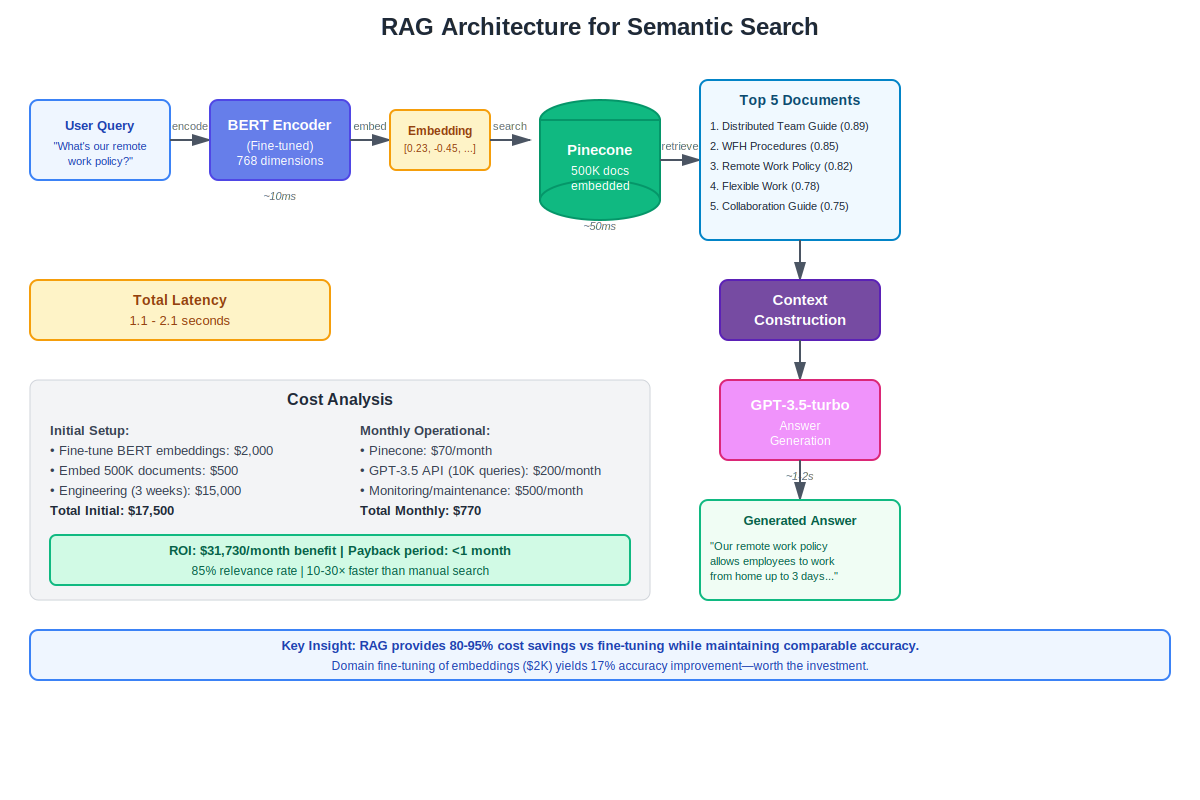
\includegraphics[width=0.95\textwidth]{chapters/diagrams/chapter10_rag_semantic_search_a1b2c3d4.pdf}
\caption{RAG architecture for semantic search showing query encoding, vector retrieval, and answer generation with timing and cost breakdown. The pipeline demonstrates how BERT embeddings, Pinecone vector search, and GPT-3.5 combine to deliver sub-2-second responses at \$770 monthly operational cost.}
\label{fig:rag_semantic_search}
\end{figure}

\subsection{Implementation, Governance, and Results}

The implementation pipeline processes queries through four sequential stages. Query encoding takes approximately 10 milliseconds, transforming the natural language query into a 768-dimensional embedding vector. Vector search against the Pinecone index takes approximately 50 milliseconds, returning the top 5 most similar document chunks with similarity scores. Context construction concatenates the retrieved chunks into a single prompt, taking negligible time. Answer generation via GPT-3.5-turbo takes 1--2 seconds, producing a natural language response with source citations.

Total latency ranges from 1.1 to 2.1 seconds, meeting the sub-second perceived latency requirement when combined with progressive UI updates. The system displays retrieved documents immediately while the answer generates, providing users with useful information even before the generated answer appears.

Governance considerations are embedded into the architecture rather than added as an afterthought. Access control is enforced at retrieval time: the vector index stores document-level access metadata, and queries include user identity and roles. The retrieval layer filters candidates to those the user is permitted to access before similarity ranking. Audit logs capture which documents were retrieved for which queries, who viewed them, and which documents contributed to generated answers. These logs support internal audits and regulatory inquiries.


Performance metrics demonstrate substantial improvement over keyword search. Relevant results in the top 5 increase from 45\% to 85\%---an 89\% improvement. Time to find answers decreases from 5--10 minutes to 10--30 seconds---a 10--30\times speedup. Employee satisfaction scores increase from 3.2 to 4.5 out of 5. Support ticket volume decreases by roughly 60\%, from 500 to 200 weekly, as employees find answers independently.

The cost structure divides into initial setup and ongoing operational expenses. Initial setup includes approximately \$2,000 for fine-tuning BERT embeddings, \$500 for embedding the initial 500,000 documents, and \$15,000 for three weeks of engineering effort---totaling \$17,500. Monthly operational costs include \$70 for Pinecone, \$200 for GPT-3.5 API usage at 10,000 queries monthly, and \$500 for monitoring, governance reporting, and maintenance---totaling \$770 monthly.

Return on investment calculation reveals rapid payback. Cost avoidance from 300 fewer support tickets weekly, at 30 minutes per ticket and \$50 hourly labor cost, yields \$7,500 monthly savings. Productivity gains from 1,000 employees saving 30 minutes monthly at \$50 hourly cost yields \$25,000 monthly savings. Total monthly benefit reaches approximately \$31,730 against \$770 operational cost, providing a payback period under one month for the \$17,500 initial investment.

\subsection{Lessons and Considerations}

Several lessons emerge from this implementation. Domain fine-tuning proves worth the investment despite the compute cost and engineering effort. The 17 percentage point accuracy improvement translates directly to user satisfaction and adoption. Organizations deploying semantic search in specialized domains should budget for fine-tuning and treat it as part of the core project, not an optional enhancement.

Managed services provide better economics than self-hosting at startup and mid-scale. The engineering effort required for self-hosted vector databases---setup, monitoring, scaling, backup---exceeds the cost savings until reaching multi-million vector scale and mature operations. Organizations should default to managed services unless scale or data residency requirements clearly justify self-hosting investment.

Model selection should prioritize cost-performance ratio and governance constraints over absolute performance. GPT-3.5 provides 95\% of GPT-4's quality at 10\% of the cost for this application, and can often be deployed within a broader compliance perimeter faster than newer models. The modest quality gap rarely justifies 10\times cost increase. Organizations should test whether smaller, cheaper models suffice before defaulting to the largest available models.

Chunk size optimization requires empirical testing with representative queries and documents. Optimal configuration depends on document structure, query types, and retrieval precision requirements. Organizations should test multiple configurations rather than assuming a default chunk size and should validate that chunking respects access control and sensitivity boundaries.

Embedding refresh requirements often exceed initial estimates. Documents change---policies update, procedures evolve, new content is added. Stale embeddings degrade retrieval quality over time. Organizations should plan for regular re-embedding of changed documents and periodic full re-embedding to maintain quality, and should ensure that re-embedding workflows comply with data retention and audit requirements.

\section{Customer Support Automation}

\subsection{Business Context and Requirements}

Customer support represents a high-volume, high-cost operation for most organizations. Support teams handle thousands of inquiries daily, many addressing common questions answerable from documentation or standard procedures. Human agents cost \$25--50 per hour including overhead. Average handling time ranges from 5--15 minutes per inquiry. Monthly support costs for organizations handling 100,000 inquiries reach \$200,000--500,000.

Conversational AI promises to automate routine inquiries, reducing costs while maintaining or improving response quality and latency. The business case requires demonstrating that automated responses achieve acceptable accuracy---typically 85\%+ for tier-1 support---while reducing per-inquiry costs by 80\%+ compared to human agents. The system must handle conversation context, access knowledge bases, escalate complex issues to human agents, and integrate with existing ticketing systems, authentication, and CRM platforms.

Technical requirements include sub-3-second response latency, support for multi-turn conversations with context retention, access to 10,000+ knowledge base articles, and graceful degradation when confidence is low. The system must handle 100,000 conversations monthly with operational costs under roughly \$5,000 monthly to achieve target cost reduction. Governance requirements include logging all interactions, preserving escalation trails, and being able to demonstrate how responses were generated when customer disputes or regulatory inquiries arise.

\subsection{Architecture and Technical Decisions}

The architecture combines conversational AI with retrieval-augmented generation and selective context management. The system maintains conversation state, retrieves relevant knowledge base articles, and generates contextually appropriate responses. Key technical decisions determine cost, performance, and compliance characteristics.

Context window management proves critical for cost control. The initial proposal suggested using GPT-4 with 32,000-token context to maintain full conversation history. At \$0.03 per 1,000 tokens for input and 100,000 conversations monthly averaging 10 exchanges, this approach costs approximately \$30,000 monthly---economically infeasible for the target cost structure.


The optimized approach uses GPT-3.5-turbo with 4,000-token context, maintaining only recent conversation history. Most support conversations require only the last 2--3 exchanges for context---earlier messages rarely influence current responses. When full conversation history proves necessary, the system retrieves it from the conversation database rather than including it in every API call. This selective context management reduces average token consumption from roughly 30,000 to 2,000 per conversation.

The cost calculation reveals dramatic savings. GPT-3.5-turbo costs approximately \$0.001 per 1,000 input tokens and \$0.002 per 1,000 output tokens. An average conversation consumes 2,000 input tokens and 500 output tokens, costing about \$0.003 per conversation. At 100,000 conversations monthly, total API cost reaches \$300---a 99\% reduction from the initial \$30,000 estimate. This cost structure makes the business case compelling while meeting latency targets.

Knowledge base integration uses the same RAG pattern as semantic search. Customer inquiries encode into embeddings, retrieve relevant knowledge base articles, and include them as context for response generation. The vector database contains embeddings for approximately 10,000 knowledge base articles, costing around \$15 monthly for Pinecone hosting at this scale. Retrieval adds 50--100 milliseconds to response latency---acceptable given the 2-second response target.

Confidence scoring enables intelligent escalation. The system evaluates response confidence based on retrieval similarity scores and signals from the model output. Low-confidence responses trigger human escalation rather than providing potentially incorrect information. The threshold calibration---typically 0.7--0.8 similarity score---balances automation rate against accuracy. Higher thresholds increase accuracy but reduce automation; lower thresholds increase automation but risk more errors. Governance processes define which categories of inquiries must always escalate regardless of confidence (for example, billing disputes or regulatory complaints).

Conversation state management requires careful engineering. The system stores conversation history in a database, maintaining user context across sessions. Each message includes metadata---timestamp, user ID, confidence scores, knowledge base articles referenced, escalation decisions---enabling analytics and quality monitoring. The state management adds approximately 20 milliseconds to response latency for database operations, and the database becomes part of the compliance boundary because it contains full interaction history.

\begin{figure}[htbp]
\centering
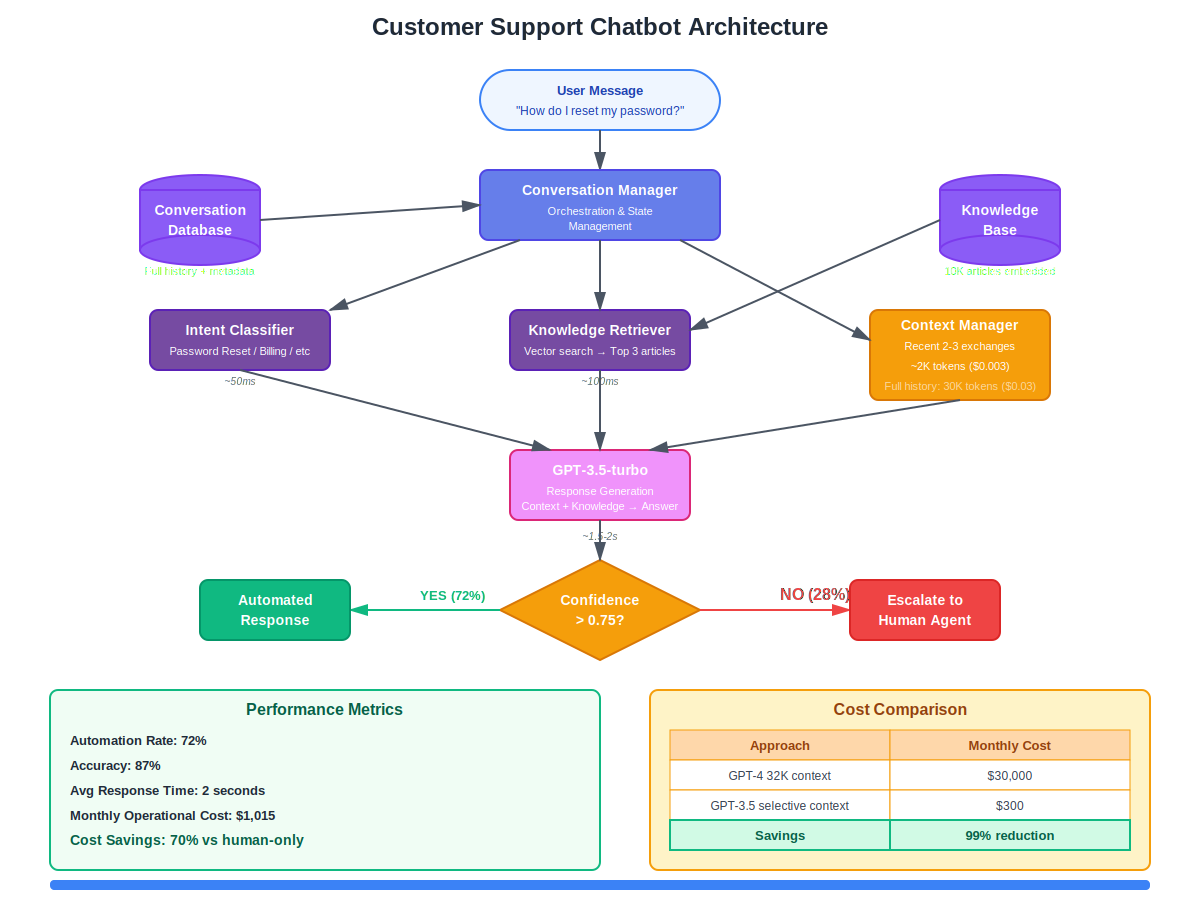
\includegraphics[width=0.95\textwidth]{chapters/diagrams/chapter10_chatbot_architecture_e5f6g7h8.pdf}
\caption{Customer support chatbot architecture with selective context management and confidence-based escalation. The system achieves 72\% automation rate and 99\% cost reduction through intelligent context window management (2K vs 30K tokens) and hybrid human-AI workflows.}
\label{fig:chatbot_architecture}
\end{figure}

\subsection{Implementation, Operations, and Results}

The implementation architecture consists of several integrated components. The conversation manager maintains state and orchestrates the pipeline. The intent classifier determines query type and routes to appropriate handlers. The knowledge retriever searches the vector database for relevant articles. The response generator produces natural language responses using GPT-3.5-turbo with retrieved context. The confidence evaluator scores responses and triggers escalation when necessary.

Response latency breaks down across components: intent classification takes around 50 milliseconds, knowledge retrieval takes 100 milliseconds, response generation takes 1.5--2 seconds, and database operations take about 50 milliseconds. Total latency ranges from 1.7 to 2.2 seconds, meeting the sub-3-second requirement.

Performance metrics demonstrate strong business impact. Automation rate reaches 72\%---72,000 of 100,000 monthly inquiries handled without human intervention. Automated response accuracy measures 87\% based on user feedback and quality audits. Average response time decreases from roughly 8 minutes with human agents to approximately 2 seconds with automation. Customer satisfaction scores remain stable at 4.2 out of 5, indicating that automation maintains service quality.

Cost analysis reveals substantial savings. Monthly operational costs include \$300 for GPT-3.5 API usage, \$15 for Pinecone vector database, \$200 for conversation database hosting, and \$500 for monitoring, governance reporting, and maintenance---totaling \$1,015 monthly. Human agent costs for the 28,000 inquiries requiring escalation, at 10 minutes average handling time and \$40 hourly cost, total \$18,667 monthly. Combined monthly cost reaches approximately \$19,682.

Comparing to the baseline of 100,000 inquiries handled entirely by human agents at 10 minutes average and \$40 hourly cost yields roughly \$66,667 monthly. The automated system reduces costs by about 70\%, saving \$46,985 monthly or \$563,820 annually. Initial development costs of around \$50,000 pay back in just over one month.

Operational reality introduces additional considerations. Quality monitoring reveals that automated responses perform best for procedural questions with clear answers in documentation---password resets, account status checks, policy clarifications. Performance degrades for complex troubleshooting, emotional situations, and edge cases not covered in documentation. The system correctly escalates most complex cases, though approximately 5\% of automated responses should have escalated but did not, requiring subsequent human intervention. Governance teams use these metrics to refine escalation thresholds and update knowledge base content.

\subsection{Lessons and Considerations}

Context window management represents the primary cost driver for conversational AI. Organizations should carefully analyze how much context each interaction truly requires rather than defaulting to maximum context windows. Most conversations need only recent history, with full history retrievable on demand. This selective approach reduces costs by more than 90\% while maintaining quality.


Model selection should match task requirements and governance constraints. GPT-4 provides marginal quality improvements for straightforward support inquiries but costs 10--20\times more than GPT-3.5. In many enterprise cases, the slight quality improvement does not justify the cost and may introduce additional compliance review requirements. Organizations should test whether smaller models suffice before committing to expensive models. The cost difference compounds across millions of interactions.

Confidence-based escalation proves essential for maintaining quality. Attempting to automate all inquiries regardless of confidence leads to poor customer experiences and erodes trust. Organizations should calibrate escalation thresholds based on the cost of errors versus the cost of human handling. High-stakes domains (for example, financial commitments or regulatory complaints) require higher thresholds; low-stakes domains can tolerate lower thresholds.

Knowledge base quality determines automation success more than model sophistication. Well-organized, comprehensive, up-to-date documentation enables high automation rates with simple retrieval. Poor documentation limits automation regardless of model capability. Organizations should invest in knowledge base improvement before or alongside automation implementation. Governance teams should treat knowledge base maintenance as an ongoing operational responsibility, not a one-time project.

Continuous monitoring and improvement prove necessary for sustained performance. Customer language evolves, new products launch, policies change. The system requires ongoing tuning---updating knowledge bases, refining retrieval, adjusting confidence thresholds. Organizations should budget for continuous improvement rather than treating deployment as a one-time project.

Integration complexity often exceeds initial estimates. Connecting with ticketing systems, CRM platforms, authentication services, and analytics tools requires substantial engineering effort. Organizations should allocate 40--60\% of project time to integration and governance rather than focusing solely on the AI components.

\section{Classification and Categorization Systems}

\subsection{Business Context and Requirements}

Classification is one of the most common and economically valuable NLP patterns in enterprise environments. Many workflows begin with assigning a category, label, or priority to an incoming item: routing customer emails to the correct team, determining the topic of a support ticket, assigning risk levels to contracts, or classifying documents for retention and compliance. These decisions directly affect workload distribution, response times, and risk exposure.

Unlike semantic search and conversational systems, classification typically produces structured outputs drawn from a predefined label set. This structure aligns well with downstream workflow engines and reporting systems. However, accuracy requirements are often stringent. Misclassifying a high-priority complaint as low-priority may breach service-level agreements; misclassifying a high-risk contract as low-risk may create regulatory exposure. Enterprises commonly require 90\%+ accuracy for operational classifications and 95\%+ for risk-sensitive domains.

Volume amplifies both value and risk. A service center processing 200,000 emails monthly can save thousands of agent hours if classification automates triage, but systematic misclassification can overwhelm the wrong teams or hide critical issues. Classification systems must support transparent performance monitoring, ablation testing of label definitions, and fine-grained control over thresholds and fallbacks.

\subsection{Architectural Patterns and Trade-offs}

Enterprise classification systems typically follow one of three architectural patterns: traditional supervised models, fine-tuned deep learning models, or prompt-based classification using large language models. Each pattern presents specific cost, accuracy, and governance trade-offs.

Traditional supervised models (for example, logistic regression or gradient boosting on bag-of-words or TF-IDF features) offer simplicity, low inference cost, and straightforward deployment. They require careful feature engineering and generally underperform deep learning models on nuanced language tasks, especially when label sets are large or language is informal. However, for stable, narrow domains with well-defined labels and large labeled datasets, they remain competitive and easy to explain.

Fine-tuned deep learning classifiers, typically based on transformer encoders such as BERT, deliver higher accuracy and better robustness to linguistic variation. A BERT-based classifier takes tokenized text as input and outputs label probabilities. Training requires labeled examples for each class and careful management of class imbalance. In many enterprise settings, a few thousand quality-labeled examples per class are sufficient to outperform traditional models by 5--10 percentage points in accuracy. Inference cost is higher than for traditional models but remains manageable, especially when using optimized runtimes or distilled models.

Prompt-based classification uses general-purpose LLMs with task descriptions and examples provided in the prompt. Instead of training a task-specific model, the system sends the text and an instruction such as "Classify the following email into one of: billing, technical support, sales inquiry, other". Few-shot examples in the prompt illustrate desired behavior. Prompt-based approaches eliminate model training and simplify iteration on label definitions, but per-inference cost is higher and latency depends on the LLM. For low to moderate volume applications (for example, up to tens of thousands of items monthly), prompt-based classification can be economically attractive; for high-volume flows, fine-tuning becomes more cost-effective.


\subsection{Implementation Example: Email Triage}

Consider a financial services organization receiving 150,000 customer emails monthly, covering billing questions, technical support, product complaints, and regulatory requests. Historically, a manual triage team reads each email and assigns it to one of 12 queues. The average triage time is 45 seconds per email, at an effective cost of \$35 per hour. Monthly triage cost exceeds \$65,000, and misrouted emails introduce additional handling delays.

A BERT-based classifier is trained to automate triage. The project team assembles a labeled dataset of 60,000 historical emails with triage labels drawn from production ticketing systems. After cleaning and balancing classes, 50,000 emails are used for training and 10,000 for validation and testing. Training on a single GPU completes in under 6 hours, including hyperparameter tuning, at a direct compute cost under \$500.

The trained classifier achieves 93\% overall accuracy on the test set and above 95\% accuracy on high-volume classes such as billing and technical support. For low-volume, high-risk classes---for example, "regulatory complaint"---accuracy is lower, and misclassifications carry higher cost. The system therefore applies a hybrid strategy: predictions with confidence above 0.9 are auto-routed; predictions between 0.6 and 0.9 go to a reduced manual triage queue; predictions below 0.6 are treated as uncertain and require full review.

Inference is deployed as a stateless microservice with an optimized BERT variant. Average inference latency is 15 milliseconds per email, and serving costs on a modest GPU-backed instance amount to approximately \$400 monthly. With the hybrid strategy, 80\% of emails are auto-routed, 15\% go through partial review, and 5\% require full triage. Manual effort drops by more than 60\%, cutting monthly triage cost from \$65,000 to roughly \$25,000 while improving response times.

From a governance perspective, the classifier's behavior is monitored continuously. Confusion matrices by class are calculated weekly; drifts in class distribution or accuracy trigger re-training. Audit logs record which model version produced each routing decision, supporting later investigations. Label definitions and threshold policies are documented and reviewed with compliance teams, ensuring that any changes go through change control.

\begin{figure}[htbp]
\centering
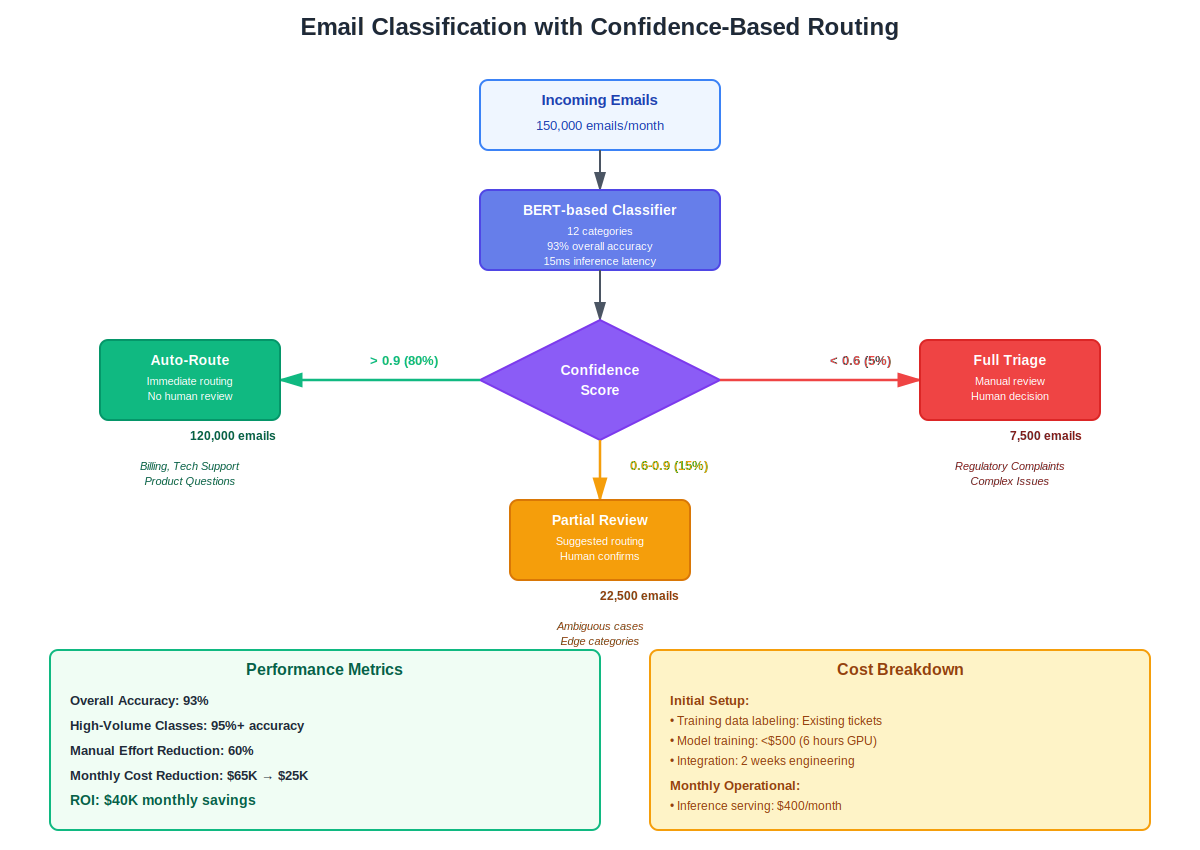
\includegraphics[width=0.95\textwidth]{chapters/diagrams/chapter10_classification_triage_i9j0k1l2.pdf}
\caption{Email classification with confidence-based routing showing hybrid automation strategy. High-confidence predictions (80\%) are auto-routed, medium-confidence (15\%) receive partial review, and low-confidence (5\%) require full manual triage. This approach achieves 60\% manual effort reduction while maintaining quality for high-risk categories.}
\label{fig:classification_triage}
\end{figure}

\subsection{Prompt-based Classification for Low-Volume Flows}

For lower-volume, higher-complexity flows, prompt-based classification may be preferable to fine-tuning. Suppose the same organization wants to classify a smaller stream of executive-level correspondence, averaging 3,000 emails monthly, into nuanced categories such as "strategic partnership opportunity", "regulatory risk", "customer churn risk", and "internal escalation". The cost and complexity of building and maintaining a fine-tuned classifier may not be justified at this scale.

A GPT-3.5-based classification service can be constructed with carefully engineered prompts that describe categories and provide examples. At \$0.003 per email for input and output tokens, monthly API cost remains under \$10, and there is no training cost. Label definitions can be adjusted by editing the prompt, which is valuable when categories evolve quickly. Human review can remain in the loop for all or a subset of classifications, with LLM outputs serving as decision support rather than fully automated routing.

The trade-off is lower controllability and more variable behavior. Prompt-based classification requires more extensive monitoring for unexpected outputs, and regulatory teams may be less comfortable with systems that cannot be straightforwardly retrained on labeled data to correct systematic issues. In practice, many enterprises start with prompt-based classification for exploratory or low-volume use cases, then migrate to fine-tuned models once label definitions and value propositions stabilize.

\subsection{Lessons and Considerations}

Three lessons emerge from classification deployments. First, label design is a governance question as much as a modeling question. Overly granular labels fragment the dataset and degrade model performance; overly coarse labels reduce business value. Definitions must be co-designed with operational and compliance stakeholders and treated as living artifacts.

Second, performance targets must be differentiated by class. It is often acceptable if the model is less accurate on low-impact classes, provided that high-risk classes meet stringent thresholds and have conservative fallbacks. This argues for confidence-based strategies that combine automation with human review, rather than binary "automate versus not" decisions.

Third, monitoring and re-training cadence are central to maintaining performance. Changes in product offerings, communication templates, or regulatory environments alter class distributions and language patterns. Organizations should plan for periodic re-labeling and re-training, with clear ownership and budget, and should keep label taxonomies under version control to support audits.

\section{Comparative Decision Framework}

Technical leaders rarely face the question "Should we do NLP?" in the abstract. Instead, they must choose which patterns to prioritize, how to architect them, and where to accept risk. Semantic search, conversational AI, and classification address different classes of problems and exhibit different economic and governance profiles.


Semantic search with RAG excels when the primary challenge is locating information within large, mostly unstructured repositories. It provides strong explainability through source citations and can be rolled out incrementally by department or corpus. Costs are driven by embedding volume, vector storage, and generation tokens, with clear scaling characteristics. Governance complexity centers on access control and document lifecycle management.

Conversational AI delivers value when interaction volume is high and questions are repetitive. It excels at front-door triage and resolution of routine tasks, but requires careful control of hallucination risk and escalation logic. Costs are dominated by token usage and are highly sensitive to context window management and model choice. Governance focuses on interaction logging, escalation policies, and customer communication guidelines.

Classification systems provide leverage where workflows depend on routing, prioritization, or risk scoring. They integrate cleanly with workflow engines and reporting systems because outputs are structured. Their economics hinge on label design, the cost of creating labeled datasets, and serving costs for the chosen architecture (fine-tuned vs. prompt-based). Governance emphasizes label taxonomy management, threshold policies, and performance monitoring by class.

A practical decision framework considers four axes: volume, risk, structure, and governance.

\begin{itemize}
\item \textbf{Volume}: High-volume, repetitive tasks favor automation-heavy patterns such as classification and conversational AI. Lower-volume, high-value tasks may justify prompt-based approaches and heavier human-in-the-loop.
\item \textbf{Risk}: High-risk domains push systems toward RAG architectures with strong source attribution and conservative escalation, and toward hybrid patterns where automation proposes and humans confirm.
\item \textbf{Structure}: When downstream systems require structured outputs, classification or extraction is often the starting point. When the primary need is discovery and exploration, semantic search dominates.
\item \textbf{Governance Maturity}: Organizations with strong document management and access control are better positioned for semantic search and RAG. Those with mature workflow systems can absorb classification outputs more easily. Weak governance constrains NLP ambitions more than model capabilities.
\end{itemize}

Leaders evaluating enterprise NLP investments should use these axes to map candidate projects and sequence adoption. Early successes typically come from well-scoped classification or semantic search projects in domains with manageable risk and clear data ownership, building organizational confidence and governance muscle before tackling more complex conversational systems in high-stakes areas.

\section{Key Insights}

\textbf{RAG Dominates Enterprise NLP Economics}: Retrieval-augmented generation provides better cost-performance than fine-tuning for most enterprise applications where the primary task is answering questions against internal content. RAG costs 80--95\% less than fine-tuning while providing comparable or better accuracy. Updates require adding documents rather than retraining. Source attribution comes naturally. Organizations should default to RAG unless specific requirements---latency constraints, offline operation, or proprietary model needs---justify fine-tuning investment. The semantic search case study demonstrates \$770 monthly operational cost versus much higher costs for equivalent capabilities built around fine-tuned models.

\textbf{Context Window Management Drives Conversational AI Costs}: Token consumption determines API costs for conversational applications. Naive approaches using maximum context windows cost 10--100\times more than selective context management. Most conversations require only recent history---two to three exchanges---with full history retrievable on demand from a database when needed. Organizations should analyze actual context requirements rather than defaulting to maximum windows. The customer support case study demonstrates 99\% cost reduction through selective context management, from \$30,000 to \$300 monthly.

\textbf{Model Selection Should Match Task and Governance Requirements}: Larger models provide marginal quality improvements at substantial cost increases and may complicate governance. GPT-3.5 achieves 90--95\% of GPT-4's quality for factual question answering at roughly 10\% of the cost. For many enterprise applications where retrieved context provides the information and traceability is essential, smaller models suffice. Organizations should test whether smaller models meet accuracy and compliance requirements before committing to larger, more expensive models.

\textbf{Enterprise Accuracy Requirements Often Exceed Commodity Accuracy}: Accuracy levels that appear acceptable in consumer applications---for example, 80--85\%---are inadequate in regulated domains. Contract classification, medical coding, and regulatory complaint handling often require 95\%+ accuracy or conservative confidence thresholds with human review. This changes the economic calculus: many enterprise NLP systems deliberately trade automation rate for reliability and auditability, especially in high-risk classes.

\textbf{Data Governance, Not Model Capacity, Limits Scale}: In practice, the limiting factor for enterprise NLP is rarely the capacity of models; it is the quality, structure, and governance of text data. Inconsistent document repositories, weak version control, and unclear ownership lead to brittle systems, regardless of model sophistication. Organizations that invest early in document management, labeling standards, and access control see smoother scale-out and fewer production incidents.

\textbf{Integration Complexity Often Exceeds AI Complexity}: Building a proof-of-concept model is often the easiest part of an NLP project. Integrating it with identity providers, document management systems, workflow engines, and monitoring stacks consumes the majority of engineering effort. Underestimating integration complexity leads to timeline slippage and stalled deployments. Planning for 40--60\% of effort to go into integration and governance produces more realistic roadmaps.

\textbf{Confidence-Based Hybrid Patterns Maximize Value}: Pure automation is rarely optimal in enterprise NLP. Confidence-based hybrid patterns---where high-confidence cases are automated, borderline cases receive assisted triage, and low-confidence cases go to humans---deliver better economics and governance. They enable higher automation rates while respecting risk constraints and audit requirements. This pattern applies equally to semantic search (confidence-based ranking and filtering), conversational AI (escalation thresholds), and classification (auto-routing thresholds).

\textbf{Classification Provides Fast, Structured Wins}: While semantic search and conversational AI attract attention, classification systems often provide faster and more measurable returns because their outputs integrate cleanly into existing workflows. They require clearer label design and governance but can often be deployed with smaller models, lower latency, and more predictable behavior. For many organizations, classification is the most pragmatic first step into enterprise NLP.
